\documentclass[]{book}
\usepackage{lmodern}
\usepackage{amssymb,amsmath}
\usepackage{ifxetex,ifluatex}
\usepackage{fixltx2e} % provides \textsubscript
\ifnum 0\ifxetex 1\fi\ifluatex 1\fi=0 % if pdftex
  \usepackage[T1]{fontenc}
  \usepackage[utf8]{inputenc}
\else % if luatex or xelatex
  \ifxetex
    \usepackage{mathspec}
  \else
    \usepackage{fontspec}
  \fi
  \defaultfontfeatures{Ligatures=TeX,Scale=MatchLowercase}
\fi
% use upquote if available, for straight quotes in verbatim environments
\IfFileExists{upquote.sty}{\usepackage{upquote}}{}
% use microtype if available
\IfFileExists{microtype.sty}{%
\usepackage{microtype}
\UseMicrotypeSet[protrusion]{basicmath} % disable protrusion for tt fonts
}{}
\usepackage[margin=1in]{geometry}
\usepackage{hyperref}
\hypersetup{unicode=true,
            pdftitle={Defect Prediction in Software Engineering},
            pdfauthor={Daniel Rodriguez and Javier Dolado},
            pdfborder={0 0 0},
            breaklinks=true}
\urlstyle{same}  % don't use monospace font for urls
\usepackage{natbib}
\bibliographystyle{apalike}
\usepackage{color}
\usepackage{fancyvrb}
\newcommand{\VerbBar}{|}
\newcommand{\VERB}{\Verb[commandchars=\\\{\}]}
\DefineVerbatimEnvironment{Highlighting}{Verbatim}{commandchars=\\\{\}}
% Add ',fontsize=\small' for more characters per line
\usepackage{framed}
\definecolor{shadecolor}{RGB}{248,248,248}
\newenvironment{Shaded}{\begin{snugshade}}{\end{snugshade}}
\newcommand{\KeywordTok}[1]{\textcolor[rgb]{0.13,0.29,0.53}{\textbf{{#1}}}}
\newcommand{\DataTypeTok}[1]{\textcolor[rgb]{0.13,0.29,0.53}{{#1}}}
\newcommand{\DecValTok}[1]{\textcolor[rgb]{0.00,0.00,0.81}{{#1}}}
\newcommand{\BaseNTok}[1]{\textcolor[rgb]{0.00,0.00,0.81}{{#1}}}
\newcommand{\FloatTok}[1]{\textcolor[rgb]{0.00,0.00,0.81}{{#1}}}
\newcommand{\ConstantTok}[1]{\textcolor[rgb]{0.00,0.00,0.00}{{#1}}}
\newcommand{\CharTok}[1]{\textcolor[rgb]{0.31,0.60,0.02}{{#1}}}
\newcommand{\SpecialCharTok}[1]{\textcolor[rgb]{0.00,0.00,0.00}{{#1}}}
\newcommand{\StringTok}[1]{\textcolor[rgb]{0.31,0.60,0.02}{{#1}}}
\newcommand{\VerbatimStringTok}[1]{\textcolor[rgb]{0.31,0.60,0.02}{{#1}}}
\newcommand{\SpecialStringTok}[1]{\textcolor[rgb]{0.31,0.60,0.02}{{#1}}}
\newcommand{\ImportTok}[1]{{#1}}
\newcommand{\CommentTok}[1]{\textcolor[rgb]{0.56,0.35,0.01}{\textit{{#1}}}}
\newcommand{\DocumentationTok}[1]{\textcolor[rgb]{0.56,0.35,0.01}{\textbf{\textit{{#1}}}}}
\newcommand{\AnnotationTok}[1]{\textcolor[rgb]{0.56,0.35,0.01}{\textbf{\textit{{#1}}}}}
\newcommand{\CommentVarTok}[1]{\textcolor[rgb]{0.56,0.35,0.01}{\textbf{\textit{{#1}}}}}
\newcommand{\OtherTok}[1]{\textcolor[rgb]{0.56,0.35,0.01}{{#1}}}
\newcommand{\FunctionTok}[1]{\textcolor[rgb]{0.00,0.00,0.00}{{#1}}}
\newcommand{\VariableTok}[1]{\textcolor[rgb]{0.00,0.00,0.00}{{#1}}}
\newcommand{\ControlFlowTok}[1]{\textcolor[rgb]{0.13,0.29,0.53}{\textbf{{#1}}}}
\newcommand{\OperatorTok}[1]{\textcolor[rgb]{0.81,0.36,0.00}{\textbf{{#1}}}}
\newcommand{\BuiltInTok}[1]{{#1}}
\newcommand{\ExtensionTok}[1]{{#1}}
\newcommand{\PreprocessorTok}[1]{\textcolor[rgb]{0.56,0.35,0.01}{\textit{{#1}}}}
\newcommand{\AttributeTok}[1]{\textcolor[rgb]{0.77,0.63,0.00}{{#1}}}
\newcommand{\RegionMarkerTok}[1]{{#1}}
\newcommand{\InformationTok}[1]{\textcolor[rgb]{0.56,0.35,0.01}{\textbf{\textit{{#1}}}}}
\newcommand{\WarningTok}[1]{\textcolor[rgb]{0.56,0.35,0.01}{\textbf{\textit{{#1}}}}}
\newcommand{\AlertTok}[1]{\textcolor[rgb]{0.94,0.16,0.16}{{#1}}}
\newcommand{\ErrorTok}[1]{\textcolor[rgb]{0.64,0.00,0.00}{\textbf{{#1}}}}
\newcommand{\NormalTok}[1]{{#1}}
\usepackage{longtable,booktabs}
\usepackage{graphicx,grffile}
\makeatletter
\def\maxwidth{\ifdim\Gin@nat@width>\linewidth\linewidth\else\Gin@nat@width\fi}
\def\maxheight{\ifdim\Gin@nat@height>\textheight\textheight\else\Gin@nat@height\fi}
\makeatother
% Scale images if necessary, so that they will not overflow the page
% margins by default, and it is still possible to overwrite the defaults
% using explicit options in \includegraphics[width, height, ...]{}
\setkeys{Gin}{width=\maxwidth,height=\maxheight,keepaspectratio}
\IfFileExists{parskip.sty}{%
\usepackage{parskip}
}{% else
\setlength{\parindent}{0pt}
\setlength{\parskip}{6pt plus 2pt minus 1pt}
}
\setlength{\emergencystretch}{3em}  % prevent overfull lines
\providecommand{\tightlist}{%
  \setlength{\itemsep}{0pt}\setlength{\parskip}{0pt}}
\setcounter{secnumdepth}{5}
% Redefines (sub)paragraphs to behave more like sections
\ifx\paragraph\undefined\else
\let\oldparagraph\paragraph
\renewcommand{\paragraph}[1]{\oldparagraph{#1}\mbox{}}
\fi
\ifx\subparagraph\undefined\else
\let\oldsubparagraph\subparagraph
\renewcommand{\subparagraph}[1]{\oldsubparagraph{#1}\mbox{}}
\fi

%%% Use protect on footnotes to avoid problems with footnotes in titles
\let\rmarkdownfootnote\footnote%
\def\footnote{\protect\rmarkdownfootnote}

%%% Change title format to be more compact
\usepackage{titling}

% Create subtitle command for use in maketitle
\newcommand{\subtitle}[1]{
  \posttitle{
    \begin{center}\large#1\end{center}
    }
}

\setlength{\droptitle}{-2em}
  \title{Defect Prediction in Software Engineering}
  \pretitle{\vspace{\droptitle}\centering\huge}
  \posttitle{\par}
  \author{Daniel Rodriguez and Javier Dolado}
  \preauthor{\centering\large\emph}
  \postauthor{\par}
  \predate{\centering\large\emph}
  \postdate{\par}
  \date{2017-06-24}

\usepackage{booktabs}

\usepackage{amsthm}
\newtheorem{theorem}{Theorem}[chapter]
\newtheorem{lemma}{Lemma}[chapter]
\theoremstyle{definition}
\newtheorem{definition}{Definition}[chapter]
\newtheorem{corollary}{Corollary}[chapter]
\newtheorem{proposition}{Proposition}[chapter]
\theoremstyle{definition}
\newtheorem{example}{Example}[chapter]
\theoremstyle{remark}
\newtheorem*{remark}{Remark}
\begin{document}
\maketitle

{
\setcounter{tocdepth}{1}
\tableofcontents
}
\chapter*{Welcome}\label{welcome}
\addcontentsline{toc}{chapter}{Welcome}

Defect Prediction in Software Engineering. Work in progress.

This work is licensed under the
\href{http://creativecommons.org/licenses/by-nc-nd/3.0/us/}{Creative
Commons Attribution-NonCommercial-NoDerivs 3.0} United States License.

\part{Introduction to Defect Prediction in Software
Engineering}\label{part-introduction-to-defect-prediction-in-software-engineering}

Defect Prediction in Data Mining

Defect Classification

Defect Prediction and Ranking

Standards to deal with defects

ODC (Orthogonal defect classification)

AutoODC

\part{Data Sources in Software Engineering in Software
Engineering}\label{part-data-sources-in-software-engineering-in-software-engineering}

\chapter{Data Sources in Software
Engineering}\label{data-sources-in-software-engineering}

We classify this trail in the following categories:

\begin{itemize}
\item
  \emph{Source code} can be studied to measure its properties, such as
  size or complexity.
\item
  \emph{Source Code Management Systems} (SCM) make it possible to store
  all the changes that the different source code files undergo during
  the project. Also, SCM systems allow for work to be done in parallel
  by different developers over the same source code tree. Every change
  recorded in the system is accompanied with meta-information (author,
  date, reason for the change, etc) that can be used for research
  purposes.
\item
  \emph{Issue or Bug tracking systems} (ITS). Bugs, defects and user
  requests are managed in ISTs, where users and developers can fill
  tickets with a description of a defect found, or a desired new
  functionality. All the changes to the ticket are recorded in the
  system, and most of the systems also record the comments and
  communications among all the users and developers implied in the task.
\item
  \emph{Messages} between developers and users. In the case of free/open
  source software, the projects are open to the world, and the messages
  are archived in the form of mailing lists and social networks which
  can also be mined for research purposes. There are also some other
  open message systems, such as IRC or forums.
\item
  \emph{Meta-data about the projects}. As well as the low level
  information of the software processes, we can also find meta-data
  about the software projects which can be useful for research. This
  meta-data may include intended-audience, programming language, domain
  of application, license (in the case of open source), etc.
\item
  \emph{Usage data}. There are statistics about software downloads, logs
  from servers, software reviews, etc.
\end{itemize}

\section{Types of information stored in the
repositories}\label{types-of-information-stored-in-the-repositories}

\begin{itemize}
\item
  Meta-information about the project itself and the people that
  participated.

  \begin{itemize}
  \item
    Low-level information

    \begin{itemize}
    \item
      Mailing Lists (ML)
    \item
      Bugs Tracking Systems (BTS) or Project Tracker System (PTS)
    \item
      Software Configuration Management Systems (SCM)
    \end{itemize}
  \item
    Processed information. For example project management information
    about the effort estimation and cost of the project.
  \end{itemize}
\item
  Whether the repository is public or not
\item
  Single project vs.~multiprojects. Whether the repository contains
  information of a single project with multiples versions or multiples
  projects and/or versions.
\item
  Type of content, open source or industrial projects
\item
  Format in which the information is stored and formats or technologies
  for accessing the information:

  \begin{itemize}
  \item
    Text. It can be just plain text, CSV (Comma Separated Values) files,
    Attribute-Relation File Format (ARFF) or its variants
  \item
    Through databases. Downloading dumps of the database.
  \item
    Remote access such as APIs of Web services or REST
  \end{itemize}
\end{itemize}

\chapter{Repositories}\label{repositories}

There is a number of open research repositories in Software Engineering.
Among them:

\begin{itemize}
\item
  FLOSSMole \citep{HCC06} \url{http://flossmole.org/}
\item
  FLOSSMetrics \citep{herraiz2009flossmetrics}:
  \url{http://flossmetrics.org/}
\item
  PROMISE (PRedictOr Models In Software Engineering) {[}8{]}:
  \url{http://openscience.us/repo/}
\item
  Qualitas Corpus (QC) \citep{QualitasCorpus2010}:
  \url{http://qualitascorpus.com/}
\item
  Sourcerer Project \citep{LBNRB09}: \url{http://sourcerer.ics.uci.edu/}
\item
  Ultimate Debian Database (UDD) \citep{NZ10}
  \url{http://udd.debian.org/}
\item
  SourceForge Research Data Archive (SRDA) \citep{VanAntwerpM2008}
  \url{http://zerlot.cse.nd.edu/}
\item
  SECOLD (Source code ECOsystem Linked Data):
  \url{http://www.secold.org/}
\item
  Software-artifact Infrastructure Repository (SIR)
  {[}\url{http://sir.unl.edu}{]}
\item
  OpenHub: \url{https://www.openhub.net/}
\end{itemize}

Not openly available:

\begin{itemize}
\item
  The International Software Benchmarking Standards Group (ISBSG)
  \url{http://www.isbsg.org/}
\item
  TukuTuku \url{http://www.metriq.biz/tukutuku/}
\end{itemize}

Some papers and publications/theses that have been used in the
literature:

\begin{itemize}
\item
  Helix Data Set \citep{Vasa2010}:
  \url{http://www.ict.swin.edu.au/research/projects/helix/}
\item
  Bug Prediction Dataset (BPD) \citep[\citet{ALR11}]{DAmb2010a}:
  \url{http://bug.inf.usi.ch/}
\item
  Eclipse Bug Data (EBD) \citep[\citet{NZZH12}]{ZPZ07}:
  \url{http://www.st.cs.uni-saarland.de/softevo/bug-data/eclipse/}
\end{itemize}

\section{Some Tools/Dashboards to extract
data}\label{some-toolsdashboards-to-extract-data}

Within the open source community, two toolkits allow us to extract data
that can be used to explore projects:

Metrics Grimoire \url{http://metricsgrimoire.github.io/}

SonarQube \url{http://www.sonarqube.org/}

\chapter{Metrics in Soft Eng
Prediction}\label{metrics-in-soft-eng-prediction}

\section{Complexity Metrics}\label{complexity-metrics}

These metrics have been used for quality assurance during:

\begin{itemize}
\tightlist
\item
  Development to obtain quality measures, code reviews etc.
\item
  Testing to focus and prioritize testing effort, improve efficiency
  etc.
\item
  Maintenance as indicators of comprehensibility of the modules etc.
\end{itemize}

Generally, the developers or maintainers use rules of thumb or threshold
values to keep modules, methods etc. within certain range. For example,
if the cyclomatic complexity (\(v(g)\)) of a module is between 1 and 10,
it is considered to have a very low risk of being defective; however,
any value greater than 50 is considered to have an unmanageable
complexity and risk. For the essential complexity (\(ev(g)\)), the
threshold suggested is 4 etc. Although these metrics have been used for
long time, there are no clear thresholds, for example, although McCabe
suggests a threshold of 10 for \(v(g)\), NASA's in--house studies for
this metric concluded that a threshold of 20 can be a better predictor
of a module being defective.

Several authors have studied the relation between lines of code and
defects, for example, \citep{Zhang2009}

\subsection{McCabe}\label{mccabe}

\citep{mccabe76}

\citep{Halstead77}

\begin{table}%[h!]
\small
\caption{Attribute Definition Summary}
\label{tab:attrDef}
\begin{center}
\begin{small}
\begin{tabular}{l|l|p{6cm}}
\hline
       & \emph{Metric} &  \emph{Definition} \\
\hline
\hline
    McCabe  &          $LoC$  &  McCabe's  Lines of code \\
\hline
            &       $v(g)$  &  Cyclomatic complexity \\
            &       $ev(g)$  &  Essential complexity \\
            &       $iv(g)$  &  Design complexity \\
\hline
Halstead   &     $uniqOp$  &  Unique operators, $n_1$ \\
base               &   $uniqOpnd$  &  Unique operands, $n_2$ \\
               &    $totalOp$  &  Total operators, $N_1$ \\
               &   $totalOpnd$  &  Total operands, $N_2$\\
\hline
Halstead Derived  &           n  &  Vocabulary, $n=n_1+n_2$  \\
                  &           L  &  Program length, $N = N_1 + N_2$ \\%\par {Estimated Length:} $N' = n_1\cdot log_2n_1 + n_2\cdot log_2n_2$\\
                  &           V  &  Volume, $V = N\cdot log_2(n)$ \\ %(the number of mental comparisons needed to write a program of length N)\\
                  &           d  &  Difficulty $D=1/L$\\
                  &           i  &  Intelligence \\
                  &           e  &  Effort $e=V/L$ \\ %\par estimated $e=n_1 N_2 N log_2 n / 2n_2$ (elementary mental discriminations)\\
                  &           b  &  Error Estimate \\
                  &           t  &  Time $T = E / 18$ seconds\\
                  &      lOCode  &  Line count of statement \\
                  & lOComment   &  Count of lines of comments \\
                  & lOBlank     &  Count of blank lines \\
                  & lOCodeAndComment  &  Count of lines of code and comments           \\

\hline
     Branch    &   $branchCount$  &  No. branches of the flow graph \\
\hline
     Class  &      {true, false}  &  Reported defects? \\
\hline
\end{tabular}
\end{small}
\end{center}
\end{table}

\paragraph{Halstead y su ciencia del software.-}

A finales de 1970, Halstead desarrolló un conjunto de métricas conocidas
en su conjunto como la \emph{ciencia del software de
Halstead}. Estas métricas se basan en último término en computar los
\emph{operadores} y \emph{operandos} de un programa:

\begin{itemize}
  \item Los operadores son las palabras reservadas del
  lenguaje (tales como \texttt{if}, \texttt{while} o
\texttt{for}), los operadores aritméticos (\texttt{+},
\texttt{-}, \texttt{*}, etc.), los de asignación
(\texttt{=}, \texttt{+=}, \texttt{*=}, etc.) y los
operadores lógicos (AND, OR, etc.)
  \item Los operandos son las variables, los literales y las constantes del
programa.
\end{itemize}

Halstead propone diferentes medidas que basa en el cálculo previo del
número de operadores y operandos únicos, y del número total de
operadores y operandos. Para calcular todos estos valores utiliza la
siguiente notación:

\begin{itemize}
\tightlist
\item
  \(n_1\), number of distinct operators
\item
  \(N_1\), total number of operators
\item
  \(n_2\), number of distinct operands
\item
  \(N_2\), the total number of operands
\end{itemize}

For example, given the following excerpt:

\begin{verbatim}
if (MAX < 2) {
    a = b * MAX;
    System.out.print(a);
}
\end{verbatim}

We obtain the following values:

\begin{itemize}
\tightlist
\item
  \(n1 = 6\) (if, \{ \}, System.out.print(), =, *, \(<\))
\item
  \(N1 = 6\) (if, \{ \}, System.out.print(), =, *, \(<\))
\item
  \(n2 = 4\) (MAX, a, b, 2)
\item
  \(N2 = 6\) (MAX, 2, a, b, MAX, a)
\end{itemize}

Using this four variable, several metrics are calculated.

\{Vocabulario\} (\(n = n_{1} + n_{2}\)). El vocabulario es una medida de
la complejidad de las sentencias de un programa a partir del número de
operadores y operandos únicos. Se basa en el hecho de que un programa
que utiliza un número reducido de elementos muchas veces será, según
Halstead, menos complejo que un programa que emplea un mayor número de
elementos.

\{Longitud\} (\(N = N_{1} + N_{2}\)). La longitud es una medida del
tamaño de un programa: cuanto más grande, mayor será la dificultad para
comprenderlo. Se trata de una medida alternativa a la simple cuenta de
líneas de código y casi igual de fácil de calcular. \(N\) es sin embargo
más sensible a la complejidad, porque no asume que todas las
instrucciones son igualmente fáciles o difíciles de entender. \% La
longitud puede ser estimada con la ecuación: \%
\(\hat{N} = N_{1} log_2 n_1 + N_{2} log_2 n_2\).

\{Volumen\} (\(V = N \cdot log_{2}(n)\)). El vocabulario se define como
el número de bits necesarios para codificar un programa en un alfabeto
que utiliza un único carácter para representar todo operador u operando.
Mientras que la longitud es una simple cuenta del total de operadores y
operandos, el volumen da un peso extra al número de operadores y
operandos únicos. Por ejemplo, si dos programas tienen la misma longitud
\(N\) pero uno de ellos tiene un mayor número de operadores y operandos
únicos, que naturalmente lo hacen más difícil de entender y mantener,
éste tendrá un mayor volumen.

\% Puesto que siempre \% existe un número mínimo de operadores y
operadores con los que se \% puede expresar un algoritmo, que llamaremos
\textbf{volumen
% óptimo} (\(V'\)) para representar un algoritmo. Al ratio entre \% el
volumen óptimo y el actual se denomina \% \textbf{nivel}, \(L=V'/V\).
Dado que dicho nivel es difícil \% de calcular, habitualmente se estima
mediante la ecuación: \%
\(\hat{L}= \frac{n_1'}{n_1} \cdot \frac{n_2}{N_2}\) \% \noindent donde
\(n_1'\) es el mínimo número de operadores únicos.

\item \textbf{Esfuerzo mental} (\(E = V / L\)). El esfuerzo ofrece una
estimación del trabajo requerido para desarrollar un programa dividiendo
su volumen por el nivel del lenguaje (\(L\)), siendo este \(L\) un
indicador que varía en función de si se está utilizando un lenguaje de
alto o bajo nivel. El esfuerzo crece por tanto con el volumen, pero
decrece a medida que se utiliza un lenguaje de mayor nivel. Así por
ejemplo, una llamada a un procedimiento podría tener un valor \(L = 1\)
en Java, mientras que en COBOL podría ser \(0,1\) y en lenguaje
ensamblador \(0,01\). Según estudios empíricos, \(E\) es una mejor
medida de la facilidad para comprender un programa de lo que lo es
\(N\). La motivación original de Halstead al crear esta métrica fue
representar el esfuerzo mental necesario (en términos de operaciones
mentales de discriminación) para escribir un programa de longitud \(N\).
\% Como se puede comprobar al analizar la \% fórmula anterior, \%,
siendo este \(L\) un indicador \%que varia en función de si se está
utilizando un lenguaje \%de alto o bajo nivel. \% Otra forma de calcular
el esfuerzo es: \% \(E = \frac{n_1 N_2 N log_2 n}{2 n_2}\)

\% \item \textbf{Tiempo}, \(T=E/S\), es el tiempo de desarrollo \%
medido en segundos, siendo \(S\) el número de discriminaciones \%
mentales con un valor entre \(5 \leq S \leq 20\).

\% \item \textbf{Inteligencia},
\(i = (2n_{2} / n_{1}N_{2} ) \cdot (N_{1} + % N_{2})log_{2}(n_{1} + n_{2})\),
viene a medir la funcionalidad de \% una métrica, cuanto ``dice'' un
programa. Según esta métrica, una misma función \% programada en
diferentes lenguajes debería arrojar valores \% muy similares.

\textbackslash{}end\{itemize\}

Las métricas de Halstead son tan ampliamente utilizadas como criticadas
por su comprometida validación empírica, ya que muchas de las métricas
se definen en función del número de discriminaciones mentales, un valor
ciertamente difícil de definir y validar. Debe tenerse en cuenta además
que se trata de métricas pensadas para medir programas una vez se tiene
el código completo, lo cual impide utilizarlas para realizar
estimaciones, por ejemplo. Son, sin embargo, útiles durante las
actividades de prueba pues permiten identificar aquellos módulos
potencialmente problemáticos de acuerdo a su complejidad.

\section{OO Metrics}\label{oo-metrics}

OO Metrics

\citep{Chidamber1994}

\begin{itemize}
\item
  CBO for a class is a count of the number of other classes to which it
  is coupled. Coupling between two classes is said to occur when one
  class uses methods or variables of another class. COB is measured by
  counting the number of distinct non-inheritance related class
  hierarchies on which a class depends.
\item
  DIT measures the maximum level of the inheritance hierarchy of a
  class; the root of the inheritance tree inherits from no class and is
  at level zero of the inheritance tree. Direct count of the levels of
  the levels in an inheritance hierarchy.
\item
  NOC is the number of immediate subclasses subordinate to a class in
  the hierarchy. NOC counts the number of subclasses belonging to a
  class. According to C\&K, NOC indicate the level of reuse, the
  likelihood of improper abstraction and as possible indication of the
  level of testing required.
\item
  RFC is the count of the set of all methods that can be invoked in
  response to a message to an object of the class or by some method in
  the class. This includes all methods accessible within the class
  hierarchy. RFC counts the occurrences of calls to other classes from a
  particular class. where RS is the response set for the class. The
  response set for the class can be expressed as: where \{Ri\}=set of
  methods called by method i and \{M\}=set of all methods in the class.
  The response set of a class is a set of methods that can potentially
  be executed in response to a message received by an object of that
  class. The cardinality of this set is a measure of the attributes of
  objects in the class. Since it specifically includes methods called
  from outside the class, it is also a measure of the potential
  communication between the class and other classes. According to C\&K,
  RFC is a measure of the complexity of a class through the number of
  methods and the amount of communication with other classes.
\item
  WMC measures the complexity of an individual class. If all methods are
  considered equally complex, then WMC is simply the number of methods
  defined in each class.C\&K suggests that WMC is intended to measure
  the complexity of a class. Therefore, it is an indicator of the effort
  needed to develop and maintain a class.
\item
  LCOM measures the extent to which methods reference the classes
  instance data.
\end{itemize}

\section{Process Metrics}\label{process-metrics}

Process Metrics

\section{SNA Metrics}\label{sna-metrics}

SNA Metrics

\chapter{Machine Learning in Defect
Prediction}\label{machine-learning-in-defect-prediction}

Machine Learning in Defect Prediction

\chapter{Defect Regression}\label{defect-regression}

Defect Regression

\part{Evaluation}\label{part-evaluation}

\chapter{Evaluation of Models}\label{evaluation-of-models}

Once we obtain the model with the training data, we need to evaluate it
with some new data (testing data).

We cannnot use the the same data for training and testing (it is like
evaluating a student with the exercises previouly solved.¡ in class, the
sudent's marks will be ``optimistic'' and we do not know about student
capability to generalise the learned concepts).

\section{Evaluation of Classification
Models}\label{evaluation-of-classification-models}

\subsection{Discrete Evaluation}\label{discrete-evaluation}

The confusion matrix (which can be extended to multiclass problems). The
following table shows the possible outcomes for binary classification
problems:

\begin{longtable}[]{@{}lll@{}}
\toprule
& \(Pred Pos\) & \(Pred Neg\)\tabularnewline
\midrule
\endhead
\(Act Pos\) & \(TP\) & \(FN\)\tabularnewline
\(Act Neg\) & \(FP\) & \(TN\)\tabularnewline
\bottomrule
\end{longtable}

where \emph{True Positives} (\(TP\)) and \emph{True Negatives} (\(TN\))
are respectively the number of positive and negative instances correctly
classified, \emph{False Positives} (\(FP\)) is the number of negative
instances misclassified as positive (also called Type I errors), and
\emph{False Negatives} (\(FN\)) is the number of positive instances
misclassified as negative (Type II errors).

From the confusion matrix, we can calculate:

\begin{itemize}
\tightlist
\item
  \emph{True positive rate}, or \emph{recall }
  \(TP_r = recall = r = TP/TP+FN\) is the proportion of positive cases
  correctly classified as belonging to the positive class.
\item
  \emph{False negative rate} (\(FN_r=FN/TP+FN\)) is the proportion of
  positive cases misclassified as belonging to the negative class.
\item
  \emph{False positive rate} (\(FP_r=FP/FP+TN\)) is the proportion of
  negative cases misclassified as belonging to the positive class.
\item
  \emph{True negative rate} (\(TN_r=TN/FP+TN\)) is the proportion of
  negative cases correctly classified as belonging to the negative
  class.
\end{itemize}

There is a tradeoff between \(FP_r\) and \(FN_r\) as the objective is
minimize both metrics (or conversely, maximize the true negative and
positive rates). It is possible to combine both metrics into a single
figure, predictive \(accuracy\):

(\(accuracy = \frac{TP + TN}{TP + TN + FP + FN}\))

to measure performance of classifiers (or the complementary value, the
error rate\} which is defined as \(1-accuracy\))

f-measure

G-mean

\(\sqrt{PD \times Precision}\)

G-mean2

\(\sqrt{PD \times Specificity}\)

j-coeff = sensitivity + specificity - 1 = PD -PF

(Jiang, Cubic and Ma, 2008 ESE)

\begin{quote}
\textbf{No Free Lunch theorem} In the absence of any knowledge about the
prediction problem, no model can be said to be uniformly better than any
other
\end{quote}

\subsection{Prediction in probabilistic
classifiers}\label{prediction-in-probabilistic-classifiers}

A probabilistic classifier estimates the probability of each of the
posible class values given the attribute values of the instance
\(P(c|{x})\). Then, given a new instance, \({x}\), the class value with
the highest a posteriori probability will be assigned to that new
instance (the \emph{winner takes all} approach):

\(\psi({x}) = argmax_c (P(c|{x}))\)

\subsection{Metrics used in Software Engineering and Defect
Classification}\label{metrics-used-in-software-engineering-and-defect-classification}

In the domain of defect prediction and when two classes are considered,
it is also customary to refer to the \emph{probability of detection},
(\(pd\)) which corresponds to the True Positive rate (\(TP_{rate}\) or
\emph{Sensitivity}) as a measure of the goodness of the model, and
\emph{probability of false alarm} (\(pf\)) as performance
measures\textasciitilde{}\cite{Menzies07}.

The objective is to find which techniques that maximise \(pd\) and
minimise \(pf\). As stated by Menzies et al., the balance between these
two measures depends on the project characteristics (e.g.~real-time
systems vs.~information management systems) it is formulated as the
Euclidean distance from the sweet spot \(pf=0\) and \(pd=1\) to a pair
of \((pf,pd)\).

\(balance=1-\frac{\sqrt{(0-pf^2)+(1-pd^2)}}{\sqrt{2}}\)

It is normalized by the maximum possible distance across the ROC square
(\(\sqrt{2}, 2\)), subtracted this value from 1, and expressed it as a
percentage.

\subsection{Numeric Prediction
Evaluation}\label{numeric-prediction-evaluation}

RSME Mean Square Error = \(MSE\) =
\(\frac{(p_1-a_1)^2 + \ldots +(p_n-a_n)^2}{n}\)

\({MSE}=\frac{1}{n}\sum_{i=1}^n(\hat{y_i} - y_i)^2\)

\({RMSD}=\sqrt{\frac{\sum_{t=1}^n (\hat y_t - y)^2}{n}}\)

A suitable and interesting performance metric for binary classification
when data are imbalanced is the Matthew's Correlation Coefficient
(\(MCC\))\textasciitilde{}\cite{Matthews1975Comparison}:

\(MCC=\frac{TP\times TN - FP\times FN}{\sqrt{(TP+FP)(TP+FN)(TN+FP)(TN+FN)}}\)

\(MCC\) can also be calculated from the confusion matrix. Its range goes
from -1 to +1; the closer to one the better as it indicates perfect
prediction whereas a value of 0 means that classification is not better
than random prediction and negative values mean that predictions are
worst than random.

Mean-absolute error \(MAE\)

\(\frac{|p_1-a_1| + \ldots +|p_n-a_n|}{n}\)

Relative absolute error:

\(RAE = \frac{ \sum^N_{i=1} | \hat{\theta}_i - \theta_i | } { \sum^N_{i=1} | \overline{\theta} - \theta_i | }\)

Root relative-squared error:

\(RAE = \sqrt{ \frac{ \sum^N_{i=1} | \hat{\theta}_i - \theta_i | } { \sum^N_{i=1} | \overline{\theta} - \theta_i | } }\)

where \(\hat{\theta}\) is a mean value of \(\theta\).

Relative-squared error
\(\frac{(p_1-a_1)^2 + \ldots +(p_n-a_n)^2}{(a_1-\hat{a})^2 + \ldots + (a_n-\hat{a})^2}\)
(\(\hat{a}\) is the mean value over the training data)

Relative Absolut Error

Correlation Coefficient

Correlation coefficient between two random variables \(X\) and \(Y\) is
defined as \[\rho(X,Y) = \frac{{\bf
Cov}(X,Y)}{\sqrt{{\bf Var}(X){\bf Var}(Y)}}.\] The \{\em sample
correlation coefficient\} \(r\) between two samples \(x_i\) and \(y_j\)
is defined as \(r = S_{xy}/\sqrt{S_{xx}S_{yy}}.\)

Example: Is there any linear relationship between the effort estimates
(\(p_i\)) and actual effort (\(a_i\))?

\(a\|39,43,21,64,57,47,28,75,34,52\)

\(p\|65,78,52,82,92,89,73,98,56,75\)

\begin{Shaded}
\begin{Highlighting}[]
\NormalTok{p<-}\KeywordTok{c}\NormalTok{(}\DecValTok{39}\NormalTok{,}\DecValTok{43}\NormalTok{,}\DecValTok{21}\NormalTok{,}\DecValTok{64}\NormalTok{,}\DecValTok{57}\NormalTok{,}\DecValTok{47}\NormalTok{,}\DecValTok{28}\NormalTok{,}\DecValTok{75}\NormalTok{,}\DecValTok{34}\NormalTok{,}\DecValTok{52}\NormalTok{)}
\NormalTok{a<-}\KeywordTok{c}\NormalTok{(}\DecValTok{65}\NormalTok{,}\DecValTok{78}\NormalTok{,}\DecValTok{52}\NormalTok{,}\DecValTok{82}\NormalTok{,}\DecValTok{92}\NormalTok{,}\DecValTok{89}\NormalTok{,}\DecValTok{73}\NormalTok{,}\DecValTok{98}\NormalTok{,}\DecValTok{56}\NormalTok{,}\DecValTok{75}\NormalTok{)}
\CommentTok{#}
\KeywordTok{cor}\NormalTok{(p,a)}
\end{Highlighting}
\end{Shaded}

\begin{verbatim}
## [1] 0.8397859
\end{verbatim}

\(R^2\)

One common way to evaluate the performance of classifiers is through the
values of the confusion matrix.
Table\textasciitilde{}\ref{tab:confMatrix} shows the possible outcomes
for two classes, binary problems. \emph{True Positives} (\(TP\)) and
\emph{True Negatives} (\(TN\)) are respectively the number of positive
and negative instances correctly classified, \emph{False Positives}
(\(FP\)) is the number of negative instances misclassified as positive,
and \emph{False Negatives} (\(FN\)) is the number of positive instances
misclassified as negative.

\begin{longtable}[]{@{}ll@{}}
\toprule
TP & FN\tabularnewline
\midrule
\endhead
FP & FP\tabularnewline
\bottomrule
\end{longtable}

Based on the previously defined values:

\begin{itemize}
\tightlist
\item
  \emph{True positive rate} (\(TP_r=\frac{TP}{TP+FN}\)) is the
  proportion of positive cases correctly classified as belonging to the
  positive class.
\item
  \emph{False negative rate} (\(FN_r=\frac{FN}{TP+FN}\)) is the
  proportion of positive cases misclassified as belonging to the
  negative class.
\item
  \emph{False positive rate} (\(FP_r=\frac{FP}{FP+TN}\)) is the
  proportion of negative cases misclassified as belonging to the
  positive class.
\item
  \emph{True negative rate} (\(TN_r=\frac{TN}{FP+TN}\)) is the
  proportion of negative cases correctly classified as belonging to the
  negative class.
\end{itemize}

The range of all these metrics lies between 0 and 1 and they can be
interpreted as probabilities.

There is a trade--off between \emph{true positive rate} and
\emph{true negative rate} as the objective is to maximise both metrics.
They can be combined to form single metrics. For example, the predictive
\(accuracy\) (\(Acc\)) is defined as:
\%(Eq.\textasciitilde{}\ref{eq:accuracy})

\[
    Acc = \frac{TP + TN}{TP + TN + FP + FN}
\]

Another widely used metric when measuring the performance of classifiers
is the \(f-measure\)\textasciitilde{}\citep{WF05} as an harmonic median
of these two proportions:

\[
    f-measure = \frac{2 \cdot precision \cdot recall}{precision + recall} = \frac{2 \cdot TP}{2 \cdot TP + FP + FN}
\]

where precision (\(precision = \frac{TP}{TP+FP}\)) is the proportion of
positive predictions that are correct and \(recall\) is the \(TP_r\)
previously defined.

\section{Underfitting
vs.~Overfitting}\label{underfitting-vs.overfitting}

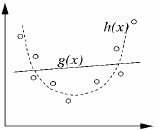
\includegraphics{figures/underfitting.png}
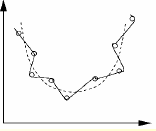
\includegraphics{figures/overfitting.png}

For example, increasing the tree size, decreases the training and
testing errors. However, at some point after (tree complexity), training
error keeps decreasing but testing error increases. Many algorithms have
parameters to determine the model complexity (e.g., in decision trees is
the prunning parameter)

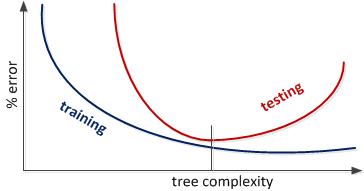
\includegraphics{figures/overfittingTrees.png} \#\# Building and
Validating a Model

\subsection{Holdout approach}\label{holdout-approach}

\textbf{Holdout approach} consists of dividing the dataset into
\emph{training} (approx. 2/3 of the data) and \emph{testing} (approx 1/3
of the data). + Problems: Data can be skewed, missing classes, etc. if
randomly divided

Stratification ensures that each class is represented with approximately
equal proportions (e.g., if data contains aprox 45\% of positive cases,
the training and testing datasets should mantain similar proportion of
positive cases).

Holdout estimate can be made more reliable by repeating the process with
different subsamples (repeated holdout method)

The error rates on the different iterations are averaged (overall error
rate)

\begin{itemize}
\tightlist
\item
  Usually, part of the data points are used for building the model and
  the remaining points are used for validating the model. There are
  several approaches to this process.
\item
  \emph{Validation Set approach}: it is the simplest method. It consists
  of randomly dividing the available set of oservations into two parts,
  a \emph{training set} and a \emph{validation set} or hold-out set.
  Usually 2/3 of the data points are used for training and 1/3 is used
  for testing purposes.
\end{itemize}

\begin{figure}[htbp]
\centering

\includegraphics{figures/validation.png}
\caption{}
\end{figure}

\section{Cross Validation (CV)}\label{cross-validation-cv}

\begin{itemize}
\item
  \emph{k-Fold Cross-Validation}: it involves randomly dividing the set
  of observations into \(k\) groups, or folds, of approximately equal
  size. The first fold is treated as a validation set, the the methods
  is fit on the remaining k-1 folds. This procedure is repeated k times.
  If k is equal to n we are in the previous method.
\item
  1st step: split dataset (\(\cal D\)) into k subsets of approximatelly
  equal size \(C_1, \dots, C_k\)
\item
  2nd step: we construct a dataset \(D_i = D-C_i\) used for training and
  test the accuracy of the classifier \(D_i\) on \(C_i\) subset for
  testing Having done this for all \(k\) we estimate the accuracy of the
  method by averaging the accuracy over the \(k\) cross-validation
  trials
\end{itemize}

\begin{figure}[htbp]
\centering
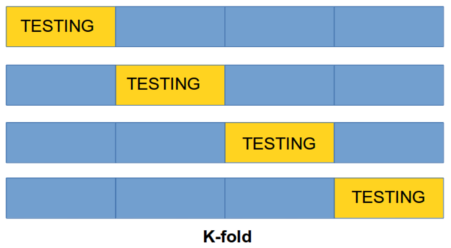
\includegraphics{figures/kfold.png}
\caption{k-fold}
\end{figure}

\begin{itemize}
\tightlist
\item
  \emph{Leave-One-Out Cross-Validation}: This is a special case of CV.
  Instead of creating two subsets for training and testing, a single
  observation is used for the validation set, and the remaining
  observations make up the training set. This approach is repeated n
  times (the total number of observations) and the estimate for the test
  mean squared error is the average of the n test estimates.
\end{itemize}

\begin{figure}[htbp]
\centering
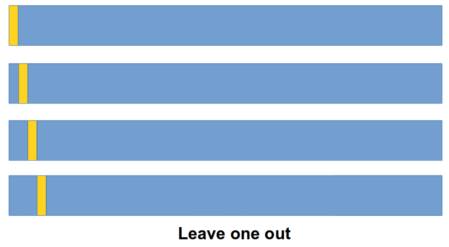
\includegraphics{figures/leaveone.png}
\caption{LOO}
\end{figure}

\subsection{China dataset. Split data into Training and
Testing}\label{china-dataset.-split-data-into-training-and-testing}

\begin{itemize}
\tightlist
\item
  The data is already divided into two different files
\end{itemize}

\begin{Shaded}
\begin{Highlighting}[]
\KeywordTok{library}\NormalTok{(foreign)}
\NormalTok{chinaTrain <-}\StringTok{ }\KeywordTok{read.arff}\NormalTok{(}\StringTok{"./datasets/effortEstimation/china3AttSelectedAFPTrain.arff"}\NormalTok{)}
\KeywordTok{nrow}\NormalTok{(chinaTrain)}
\end{Highlighting}
\end{Shaded}

\begin{verbatim}
## [1] 332
\end{verbatim}

\begin{Shaded}
\begin{Highlighting}[]
\NormalTok{logchina_size <-}\StringTok{ }\KeywordTok{log}\NormalTok{(chinaTrain$AFP)}
\NormalTok{logchina_effort <-}\StringTok{ }\KeywordTok{log}\NormalTok{(chinaTrain$Effort)}
\NormalTok{linmodel_logchina_train <-}\StringTok{ }\KeywordTok{lm}\NormalTok{(logchina_effort ~}\StringTok{ }\NormalTok{logchina_size)}
\KeywordTok{par}\NormalTok{(}\DataTypeTok{mfrow=}\KeywordTok{c}\NormalTok{(}\DecValTok{1}\NormalTok{,}\DecValTok{1}\NormalTok{))}
\KeywordTok{plot}\NormalTok{(logchina_size, logchina_effort)}
\KeywordTok{abline}\NormalTok{(linmodel_logchina_train, }\DataTypeTok{lwd=}\DecValTok{3}\NormalTok{, }\DataTypeTok{col=}\DecValTok{4}\NormalTok{)}
\end{Highlighting}
\end{Shaded}

\includegraphics{DefectPredictionSoftEng_files/figure-latex/unnamed-chunk-2-1.pdf}

\begin{Shaded}
\begin{Highlighting}[]
\KeywordTok{par}\NormalTok{(}\DataTypeTok{mfrow=}\KeywordTok{c}\NormalTok{(}\DecValTok{1}\NormalTok{,}\DecValTok{2}\NormalTok{))}
\KeywordTok{plot}\NormalTok{(linmodel_logchina_train, }\DataTypeTok{ask =} \OtherTok{FALSE}\NormalTok{)}
\end{Highlighting}
\end{Shaded}

\includegraphics{DefectPredictionSoftEng_files/figure-latex/unnamed-chunk-2-2.pdf}
\includegraphics{DefectPredictionSoftEng_files/figure-latex/unnamed-chunk-2-3.pdf}

\begin{Shaded}
\begin{Highlighting}[]
\NormalTok{linmodel_logchina_train}
\end{Highlighting}
\end{Shaded}

\begin{verbatim}
## 
## Call:
## lm(formula = logchina_effort ~ logchina_size)
## 
## Coefficients:
##   (Intercept)  logchina_size  
##        3.2485         0.7843
\end{verbatim}

\section{Graphical Evaluation}\label{graphical-evaluation}

ROC

Precision Recall

Another evaluation technique to consider when data is imbalanced is the
\emph{Receiver Operating Characteristic}
(\(ROC\))\textasciitilde{}\cite{Fawcett2006} curve which provides a
graphical visualisation of the results.

A simple way to approximate the AUC is with the following equation:
\(AUC=\frac{1+TP_{r}-FP_{r}}{2}\)

The Area Under the ROC Curve (AUC) also provides a quality measure
between positive and negative rates with a single value.

\begin{figure}[htbp]
\centering
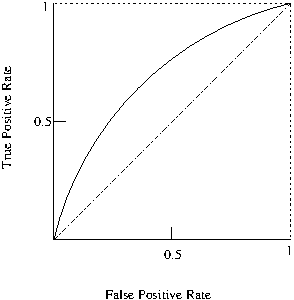
\includegraphics{figures/roc.png}
\caption{Receiver Operating Characteristic}
\end{figure}

Similarly to ROC, another widely used evaluation technique is the
Precision-Recall Curve (PRC), which depicts a trade off between
precision and recall and can also be summarised into a single value as
the Area Under the Precision-Recall Curve
(AUPRC)\textasciitilde{}\cite{Davis2006}.

\%AUPCR is more accurate than the ROC for testing performances when
dealing with imbalanced datasets as well as optimising ROC values does
not necessarily optimises AUPR values, i.e., a good classifier in AUC
space may not be so good in PRC space. \%The weighted average uses
weights proportional to class frequencies in the data. \%The weighted
average is computed by weighting the measure of class (TP rate,
precision, recall \ldots{}) by the proportion of instances there are in
that class. Computing the average can be sometimes be misleading. For
instance, if class 1 has 100 instances and you achieve a recall of 30\%,
and class 2 has 1 instance and you achieve recall of 100\% (you
predicted the only instance correctly), then when taking the average
(65\%) you will inflate the recall score because of the one instance you
predicted correctly. Taking the weighted average will give you 30.7\%,
which is much more realistic measure of the performance of the
classifier. \%NB: I gave an example with two classes, but in fact the
weighted average make sense only when you have more then two classes.
When you have only two classes weighting does not make sense, and the
measures should be computed relative to the minority class. In other
words, you are interested to know if you are able to detect the minority

\chapter{Measures of Evaluation in Software
Engineering}\label{evaluationSE}

There are several measures typically used in software engieering. In
particular for effort estimation, the following metrics are extensively
used in addition or instead of statistical measures.

\begin{itemize}
\item
  \emph{Mean of the Absolute Error (MAR)}: compute the absolute errors
  and take the mean
\item
  \emph{Geometric Mean of the Absolute Error (gMAR)}: more appropriate
  when the distribution is skewed
\item
  \emph{Mean Magnitude of the Relative Error (MMRE)}: this measure has
  been critisized many times as a biased measure
  (\(\frac{\sum_{i=1}^{n}{|{\hat{y}_i-y_i}|}/y_i}{n}\))
\item
  \emph{Median Magnitude of the Relative Error (MdMRE)}: using the
  median insted of the mean
\item
  \emph{Level of Prediction} (\(Pred(l)\)) defined as the percentage of
  estimates that are within the percentage level \(l\) of the actual
  values. The level of prediction is typically set at 25\% below and
  above the actual value and an estimation method is considered good if
  it gives a result of more than 75\%.
\item
  \emph{Standardised Accuracy (SA)} (proposed by Shepperd\&MacDonnell):
  this measure overcomes all the problems of the MMRE. It is defined as
  the MAR relative to random guessing
  (\(SA=1-{\frac{MAR}{\overline{MAR}_{P_0}}\times100}\))
\item
  \emph{Random guessing}: \(\overline{MAR}_{P_0}\) is defined as:
  predict a \(\hat{y}_t\) for the target case \emph{t} by randomly
  sampling (with equal probability) over all the remaining n-1 cases and
  take \(\hat{y}_t=y_r\) where \(r\) is drawn randomly from \(1\) to
  \(n\) and \(r\neq t\).
\item
  \emph{Exact \(\overline{MAR}_{P_0}\)}: it is an improvement over
  \(\overline{MAR}_{P_0}\). For small datasets the ``random guessing''
  can be computed exactly by iterating over all data points.
\end{itemize}

\section{Evaluation of the model in the Testing
data}\label{evaluation-of-the-model-in-the-testing-data}

\begin{Shaded}
\begin{Highlighting}[]
\KeywordTok{library}\NormalTok{(foreign)}
\NormalTok{gm_mean =}\StringTok{ }\NormalTok{function(x, }\DataTypeTok{na.rm=}\OtherTok{TRUE}\NormalTok{)\{}
  \KeywordTok{exp}\NormalTok{(}\KeywordTok{sum}\NormalTok{(}\KeywordTok{log}\NormalTok{(x[x >}\StringTok{ }\DecValTok{0}\NormalTok{]), }\DataTypeTok{na.rm=}\NormalTok{na.rm) /}\StringTok{ }\KeywordTok{length}\NormalTok{(x))\}}

\NormalTok{chinaTrain <-}\StringTok{ }\KeywordTok{read.arff}\NormalTok{(}\StringTok{"./datasets/effortEstimation/china3AttSelectedAFPTrain.arff"}\NormalTok{)}
\NormalTok{logchina_size <-}\StringTok{ }\KeywordTok{log}\NormalTok{(chinaTrain$AFP)}
\NormalTok{logchina_effort <-}\StringTok{ }\KeywordTok{log}\NormalTok{(chinaTrain$Effort)}
\NormalTok{linmodel_logchina_train <-}\StringTok{ }\KeywordTok{lm}\NormalTok{(logchina_effort ~}\StringTok{ }\NormalTok{logchina_size)}


\NormalTok{chinaTest <-}\StringTok{ }\KeywordTok{read.arff}\NormalTok{(}\StringTok{"./datasets/effortEstimation/china3AttSelectedAFPTest.arff"}\NormalTok{)}
\NormalTok{b0 <-}\StringTok{ }\NormalTok{linmodel_logchina_train$coefficients[}\DecValTok{1}\NormalTok{]}
\NormalTok{b1 <-}\StringTok{ }\NormalTok{linmodel_logchina_train$coefficients[}\DecValTok{2}\NormalTok{]}
\NormalTok{china_size_test <-}\StringTok{ }\NormalTok{chinaTest$AFP}
\NormalTok{actualEffort <-}\StringTok{ }\NormalTok{chinaTest$Effort}
\NormalTok{predEffort <-}\StringTok{ }\KeywordTok{exp}\NormalTok{(b0+b1*}\KeywordTok{log}\NormalTok{(china_size_test))}

\NormalTok{err <-}\StringTok{ }\NormalTok{actualEffort -}\StringTok{ }\NormalTok{predEffort  }\CommentTok{#error or residual}
\NormalTok{ae <-}\StringTok{ }\KeywordTok{abs}\NormalTok{(err)}
\KeywordTok{hist}\NormalTok{(ae, }\DataTypeTok{main=}\StringTok{"Absolute Error in the China Test data"}\NormalTok{)}
\end{Highlighting}
\end{Shaded}

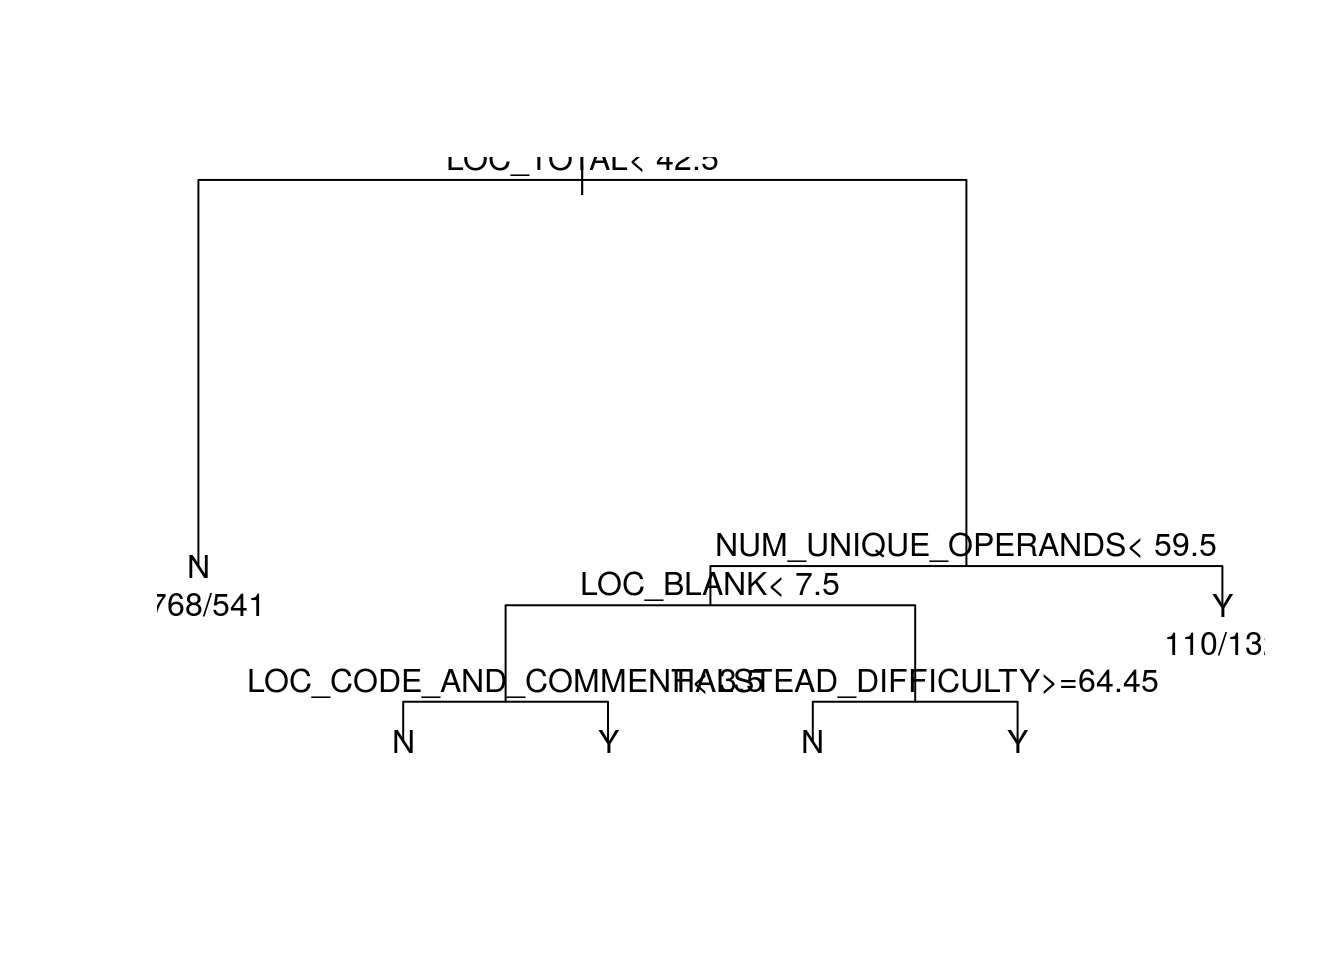
\includegraphics{DefectPredictionSoftEng_files/figure-latex/unnamed-chunk-3-1.pdf}

\begin{Shaded}
\begin{Highlighting}[]
\NormalTok{mar <-}\StringTok{ }\KeywordTok{mean}\NormalTok{(ae)}
\NormalTok{mre <-}\StringTok{ }\NormalTok{ae/actualEffort}
\NormalTok{mmre <-}\StringTok{ }\KeywordTok{mean}\NormalTok{(mre)}
\NormalTok{mdmre <-}\StringTok{ }\KeywordTok{median}\NormalTok{(mre)}
\NormalTok{gmar <-}\StringTok{ }\KeywordTok{gm_mean}\NormalTok{(ae)}
\NormalTok{mar}
\end{Highlighting}
\end{Shaded}

\begin{verbatim}
## [1] 1866.819
\end{verbatim}

\begin{Shaded}
\begin{Highlighting}[]
\NormalTok{mmre}
\end{Highlighting}
\end{Shaded}

\begin{verbatim}
## [1] 1.15106
\end{verbatim}

\begin{Shaded}
\begin{Highlighting}[]
\NormalTok{mdmre}
\end{Highlighting}
\end{Shaded}

\begin{verbatim}
## [1] 0.5510077
\end{verbatim}

\begin{Shaded}
\begin{Highlighting}[]
\NormalTok{gmar}
\end{Highlighting}
\end{Shaded}

\begin{verbatim}
## [1] 832.5504
\end{verbatim}

\begin{Shaded}
\begin{Highlighting}[]
\NormalTok{level_pred <-}\StringTok{ }\FloatTok{0.25} \CommentTok{#below and above (both)}
\NormalTok{lowpred <-}\StringTok{ }\NormalTok{actualEffort*(}\DecValTok{1}\NormalTok{-level_pred)}
\NormalTok{uppred <-}\StringTok{  }\NormalTok{actualEffort*(}\DecValTok{1}\NormalTok{+level_pred)}
\NormalTok{pred  <-}\StringTok{  }\NormalTok{predEffort <=}\StringTok{ }\NormalTok{uppred &}\StringTok{ }\NormalTok{predEffort >=}\StringTok{ }\NormalTok{lowpred  }\CommentTok{#pred is a vector with logical values }
\NormalTok{Lpred <-}\StringTok{ }\KeywordTok{sum}\NormalTok{(pred)/}\KeywordTok{length}\NormalTok{(pred)}
\NormalTok{Lpred}
\end{Highlighting}
\end{Shaded}

\begin{verbatim}
## [1] 0.1856287
\end{verbatim}

\section{Building a Linear Model on the Telecom1
dataset}\label{building-a-linear-model-on-the-telecom1-dataset}

\begin{itemize}
\tightlist
\item
  Although there are few datapoints we split the file into Train (2/3)
  and Test (1/3)
\end{itemize}

\begin{Shaded}
\begin{Highlighting}[]
\NormalTok{telecom1 <-}\StringTok{ }\KeywordTok{read.table}\NormalTok{(}\StringTok{"./datasets/effortEstimation/Telecom1.csv"}\NormalTok{, }\DataTypeTok{sep=}\StringTok{","}\NormalTok{,}\DataTypeTok{header=}\OtherTok{TRUE}\NormalTok{, }\DataTypeTok{stringsAsFactors=}\OtherTok{FALSE}\NormalTok{, }\DataTypeTok{dec =} \StringTok{"."}\NormalTok{) }\CommentTok{#read data}

\NormalTok{samplesize <-}\StringTok{ }\KeywordTok{floor}\NormalTok{(}\FloatTok{0.66}\NormalTok{*}\KeywordTok{nrow}\NormalTok{(telecom1))}
\KeywordTok{set.seed}\NormalTok{(}\DecValTok{012}\NormalTok{) }\CommentTok{# to make the partition reproducible}
\NormalTok{train_idx <-}\StringTok{ }\KeywordTok{sample}\NormalTok{(}\KeywordTok{seq_len}\NormalTok{(}\KeywordTok{nrow}\NormalTok{(telecom1)), }\DataTypeTok{size =} \NormalTok{samplesize)}
\NormalTok{telecom1_train <-}\StringTok{ }\NormalTok{telecom1[train_idx, ]}
\NormalTok{telecom1_test <-}\StringTok{ }\NormalTok{telecom1[-train_idx, ]}

\KeywordTok{par}\NormalTok{(}\DataTypeTok{mfrow=}\KeywordTok{c}\NormalTok{(}\DecValTok{1}\NormalTok{,}\DecValTok{1}\NormalTok{))}
\CommentTok{# transformation of variables to log-log}
\NormalTok{xtrain <-}\StringTok{ }\KeywordTok{log}\NormalTok{(telecom1_train$size)}
\NormalTok{ytrain <-}\StringTok{ }\KeywordTok{log}\NormalTok{(telecom1_train$effort)}
\NormalTok{lmtelecom1 <-}\StringTok{ }\KeywordTok{lm}\NormalTok{( ytrain ~}\StringTok{ }\NormalTok{xtrain)}
\KeywordTok{plot}\NormalTok{(xtrain, ytrain)}
\KeywordTok{abline}\NormalTok{(lmtelecom1, }\DataTypeTok{lwd=}\DecValTok{2}\NormalTok{, }\DataTypeTok{col=}\StringTok{"blue"}\NormalTok{)}
\end{Highlighting}
\end{Shaded}

\includegraphics{DefectPredictionSoftEng_files/figure-latex/unnamed-chunk-5-1.pdf}

\begin{Shaded}
\begin{Highlighting}[]
\NormalTok{b0_tel1 <-}\StringTok{ }\NormalTok{lmtelecom1$coefficients[}\DecValTok{1}\NormalTok{]}
\NormalTok{b1_tel1 <-}\StringTok{ }\NormalTok{lmtelecom1$coefficients[}\DecValTok{2}\NormalTok{]}
\CommentTok{# calculate residuals and predicted values}
\NormalTok{res <-}\StringTok{ }\KeywordTok{signif}\NormalTok{(}\KeywordTok{residuals}\NormalTok{(lmtelecom1), }\DecValTok{5}\NormalTok{)}

\NormalTok{xtest <-}\StringTok{ }\NormalTok{telecom1_test$size}
\NormalTok{ytest <-}\StringTok{ }\NormalTok{telecom1_test$effort}
\NormalTok{pre_tel1 <-}\StringTok{ }\KeywordTok{exp}\NormalTok{(b0+b1*}\KeywordTok{log}\NormalTok{(xtest))}
\CommentTok{# plot distances between points and the regression line}
\KeywordTok{plot}\NormalTok{(xtest, ytest)}
\KeywordTok{curve}\NormalTok{(}\KeywordTok{exp}\NormalTok{(b0_tel1+b1_tel1*}\KeywordTok{log}\NormalTok{(x)), }\DataTypeTok{from=}\DecValTok{0}\NormalTok{, }\DataTypeTok{to=}\DecValTok{300}\NormalTok{, }\DataTypeTok{add=}\OtherTok{TRUE}\NormalTok{, }\DataTypeTok{col=}\StringTok{"blue"}\NormalTok{, }\DataTypeTok{lwd=}\DecValTok{2}\NormalTok{)}
\KeywordTok{segments}\NormalTok{(xtest, ytest, xtest, pre_tel1, }\DataTypeTok{col=}\StringTok{"red"}\NormalTok{)}
\end{Highlighting}
\end{Shaded}

\includegraphics{DefectPredictionSoftEng_files/figure-latex/unnamed-chunk-5-2.pdf}

\section{Building a Linear Model on the Telecom1 dataset with all
observations}\label{building-a-linear-model-on-the-telecom1-dataset-with-all-observations}

\begin{itemize}
\tightlist
\item
  Just to visualize results
\end{itemize}

\begin{Shaded}
\begin{Highlighting}[]
\KeywordTok{par}\NormalTok{(}\DataTypeTok{mfrow=}\KeywordTok{c}\NormalTok{(}\DecValTok{1}\NormalTok{,}\DecValTok{1}\NormalTok{))}

\NormalTok{effort_telecom1 <-}\StringTok{ }\NormalTok{telecom1$effort}
\NormalTok{size_telecom1 <-}\StringTok{ }\NormalTok{telecom1$size}

\NormalTok{lmtelecom <-}\StringTok{ }\KeywordTok{lm}\NormalTok{(effort_telecom1 ~}\StringTok{ }\NormalTok{size_telecom1)}
\KeywordTok{plot}\NormalTok{(size_telecom1, effort_telecom1)}
\KeywordTok{abline}\NormalTok{(lmtelecom, }\DataTypeTok{lwd=}\DecValTok{3}\NormalTok{, }\DataTypeTok{col=}\StringTok{"blue"}\NormalTok{)}
\CommentTok{# calculate residuals and predicted values}
\NormalTok{res <-}\StringTok{ }\KeywordTok{signif}\NormalTok{(}\KeywordTok{residuals}\NormalTok{(lmtelecom), }\DecValTok{5}\NormalTok{) }
\NormalTok{predicted <-}\StringTok{ }\KeywordTok{predict}\NormalTok{(lmtelecom)}
\CommentTok{# plot distances between points and the regression line}
\KeywordTok{segments}\NormalTok{(size_telecom1, effort_telecom1, size_telecom1, predicted, }\DataTypeTok{col=}\StringTok{"red"}\NormalTok{)}

\NormalTok{level_pred <-}\StringTok{ }\FloatTok{0.25} \CommentTok{#below and above (both)}
\NormalTok{lowpred <-}\StringTok{ }\NormalTok{effort_telecom1*(}\DecValTok{1}\NormalTok{-level_pred)}
\NormalTok{uppred <-}\StringTok{  }\NormalTok{effort_telecom1*(}\DecValTok{1}\NormalTok{+level_pred)}
\NormalTok{predict_inrange  <-}\StringTok{  }\NormalTok{predicted <=}\StringTok{ }\NormalTok{uppred &}\StringTok{ }\NormalTok{predicted >=}\StringTok{ }\NormalTok{lowpred  }\CommentTok{#pred is a vector with logical values }
\NormalTok{Lpred <-}\StringTok{ }\KeywordTok{sum}\NormalTok{(predict_inrange)/}\KeywordTok{length}\NormalTok{(predict_inrange)}
\NormalTok{Lpred}
\end{Highlighting}
\end{Shaded}

\begin{verbatim}
## [1] 0.4444444
\end{verbatim}

\begin{Shaded}
\begin{Highlighting}[]
\CommentTok{#Visually plot lpred}
\KeywordTok{segments}\NormalTok{(size_telecom1, lowpred, size_telecom1, uppred, }\DataTypeTok{col=}\StringTok{"red"}\NormalTok{, }\DataTypeTok{lwd=}\DecValTok{3}\NormalTok{)}
\end{Highlighting}
\end{Shaded}

\includegraphics{DefectPredictionSoftEng_files/figure-latex/unnamed-chunk-6-1.pdf}

\begin{Shaded}
\begin{Highlighting}[]
\NormalTok{err_telecom1 <-}\StringTok{ }\KeywordTok{abs}\NormalTok{(effort_telecom1 -}\StringTok{ }\NormalTok{predicted)}
\NormalTok{mar_tel1 <-}\StringTok{ }\KeywordTok{mean}\NormalTok{(err_telecom1)}
\NormalTok{mar_tel1}
\end{Highlighting}
\end{Shaded}

\begin{verbatim}
## [1] 124.7711
\end{verbatim}

\section{Standardised Accuracy. MARP0.
ChinaTest}\label{standardised-accuracy.-marp0.-chinatest}

\begin{itemize}
\tightlist
\item
  Computing \(MARP_0\) in the China Test data
\end{itemize}

\begin{Shaded}
\begin{Highlighting}[]
\NormalTok{estimEffChinaTest <-}\StringTok{ }\NormalTok{predEffort  }\CommentTok{# This will be overwritten, no problem}
\NormalTok{numruns <-}\StringTok{ }\DecValTok{9999}
\NormalTok{randguessruns <-}\StringTok{ }\KeywordTok{rep}\NormalTok{(}\DecValTok{0}\NormalTok{, numruns)}
\NormalTok{for (i in }\DecValTok{1}\NormalTok{:numruns) \{ }
  \NormalTok{for (j in }\DecValTok{1}\NormalTok{:}\KeywordTok{length}\NormalTok{(estimEffChinaTest)) \{}
    \NormalTok{estimEffChinaTest[j] <-}\StringTok{ }\KeywordTok{sample}\NormalTok{(actualEffort[-j],}\DecValTok{1}\NormalTok{)\}}\CommentTok{#replacement with random guessingt    }
  \NormalTok{randguessruns[i] <-}\StringTok{ }\KeywordTok{mean}\NormalTok{(}\KeywordTok{abs}\NormalTok{(estimEffChinaTest-actualEffort))}
  \NormalTok{\} }
\NormalTok{marp0Chinatest <-}\StringTok{ }\KeywordTok{mean}\NormalTok{(randguessruns)}
\NormalTok{marp0Chinatest}
\end{Highlighting}
\end{Shaded}

\begin{verbatim}
## [1] 3955.782
\end{verbatim}

\begin{Shaded}
\begin{Highlighting}[]
\KeywordTok{hist}\NormalTok{(randguessruns, }\DataTypeTok{main=}\StringTok{"MARP0 distribution of the China dataset"}\NormalTok{)}
\end{Highlighting}
\end{Shaded}

\includegraphics{DefectPredictionSoftEng_files/figure-latex/unnamed-chunk-7-1.pdf}

\begin{Shaded}
\begin{Highlighting}[]
\NormalTok{saChina =}\StringTok{ }\NormalTok{(}\DecValTok{1}\NormalTok{-}\StringTok{ }\NormalTok{mar/marp0Chinatest)*}\DecValTok{100}
\NormalTok{saChina}
\end{Highlighting}
\end{Shaded}

\begin{verbatim}
## [1] 52.80784
\end{verbatim}

\section{Standardised Accuracy. MARP0.
Telecom1}\label{standardised-accuracy.-marp0.-telecom1}

\begin{itemize}
\tightlist
\item
  Computing \(MARP_0\)
\end{itemize}

\begin{Shaded}
\begin{Highlighting}[]
\NormalTok{telecom1 <-}\StringTok{ }\KeywordTok{read.table}\NormalTok{(}\StringTok{"./datasets/effortEstimation/Telecom1.csv"}\NormalTok{, }\DataTypeTok{sep=}\StringTok{","}\NormalTok{,}\DataTypeTok{header=}\OtherTok{TRUE}\NormalTok{, }\DataTypeTok{stringsAsFactors=}\OtherTok{FALSE}\NormalTok{, }\DataTypeTok{dec =} \StringTok{"."}\NormalTok{) }\CommentTok{#read data}
\CommentTok{#par(mfrow=c(1,2))}
\CommentTok{#size <- telecom1[1]$size   not needed now}
\NormalTok{actualEffTelecom1 <-}\StringTok{ }\NormalTok{telecom1[}\DecValTok{2}\NormalTok{]$effort}
\NormalTok{estimEffTelecom1 <-}\StringTok{ }\NormalTok{telecom1[}\DecValTok{3}\NormalTok{]$EstTotal }\CommentTok{# this will be overwritten}
\NormalTok{numruns <-}\StringTok{ }\DecValTok{9999}
\NormalTok{randguessruns <-}\StringTok{ }\KeywordTok{rep}\NormalTok{(}\DecValTok{0}\NormalTok{, numruns)}
\NormalTok{for (i in }\DecValTok{1}\NormalTok{:numruns) \{ }
  \NormalTok{for (j in }\DecValTok{1}\NormalTok{:}\KeywordTok{length}\NormalTok{(estimEffTelecom1)) \{}
    \NormalTok{estimEffTelecom1[j] <-}\StringTok{ }\KeywordTok{sample}\NormalTok{(actualEffTelecom1[-j],}\DecValTok{1}\NormalTok{)\}}\CommentTok{#replacement with random guessingt    }
  \NormalTok{randguessruns[i] <-}\StringTok{ }\KeywordTok{mean}\NormalTok{(}\KeywordTok{abs}\NormalTok{(estimEffTelecom1-actualEffTelecom1))}
  \NormalTok{\} }
\NormalTok{marp0telecom1 <-}\StringTok{ }\KeywordTok{mean}\NormalTok{(randguessruns)}
\NormalTok{marp0telecom1}
\end{Highlighting}
\end{Shaded}

\begin{verbatim}
## [1] 271.4162
\end{verbatim}

\begin{Shaded}
\begin{Highlighting}[]
\KeywordTok{hist}\NormalTok{(randguessruns, }\DataTypeTok{main=}\StringTok{"MARP0 distribution of the Telecom1 dataset"}\NormalTok{)}
\end{Highlighting}
\end{Shaded}

\includegraphics{DefectPredictionSoftEng_files/figure-latex/unnamed-chunk-8-1.pdf}

\begin{Shaded}
\begin{Highlighting}[]
\NormalTok{saTelecom1 <-}\StringTok{ }\NormalTok{(}\DecValTok{1}\NormalTok{-}\StringTok{ }\NormalTok{mar_tel1/marp0telecom1)*}\DecValTok{100}
\NormalTok{saTelecom1}
\end{Highlighting}
\end{Shaded}

\begin{verbatim}
## [1] 54.02961
\end{verbatim}

\subsection{MARP0 in the Atkinson
dataset}\label{marp0-in-the-atkinson-dataset}

\begin{itemize}
\tightlist
\item
  For checking results you may use figure Atkinson in
  Shepperd\&MacDonnell
\end{itemize}

\begin{verbatim}
## [1] 280.644
\end{verbatim}

\includegraphics{DefectPredictionSoftEng_files/figure-latex/unnamed-chunk-9-1.pdf}

\section{Exact MARP0}\label{exact-marp0}

\chapter{WBL simple R code to calculate Shepperd and MacDonell's marp0
exactly}\label{wbl-simple-r-code-to-calculate-shepperd-and-macdonells-marp0-exactly}

\begin{Shaded}
\begin{Highlighting}[]
\CommentTok{#example dataset}
\NormalTok{atkinson_actual_effort <-}
\StringTok{  }\KeywordTok{c}\NormalTok{(}\DecValTok{670}\NormalTok{,}\DecValTok{912}\NormalTok{,}\DecValTok{218}\NormalTok{,}\DecValTok{595}\NormalTok{,}\DecValTok{267}\NormalTok{,}\DecValTok{344}\NormalTok{,}\DecValTok{229}\NormalTok{,}\DecValTok{190}\NormalTok{,}\DecValTok{869}\NormalTok{,}\DecValTok{109}\NormalTok{,}\DecValTok{289}\NormalTok{,}\DecValTok{616}\NormalTok{,}\DecValTok{557}\NormalTok{,}\DecValTok{416}\NormalTok{,}\DecValTok{578}\NormalTok{,}\DecValTok{438}\NormalTok{)}
\NormalTok{myabs <-}\StringTok{ }\NormalTok{function(x,y) }\KeywordTok{abs}\NormalTok{(x-y)}

\CommentTok{#diffs is square array whose i,jth element = abs(actual_i - actual_j)}
\CommentTok{#in practice this is good enough but could be made more efficient by not}
\CommentTok{#explicitly storing the matrix and only using the values below the diagonal.}

\NormalTok{diffs <-}\StringTok{ }\KeywordTok{outer}\NormalTok{(atkinson_actual_effort,atkinson_actual_effort,myabs)}
\NormalTok{marp0 <-}\StringTok{ }\KeywordTok{mean}\NormalTok{(diffs)}
\NormalTok{marp0}
\end{Highlighting}
\end{Shaded}

\begin{verbatim}
## [1] 263.5078
\end{verbatim}

\begin{Shaded}
\begin{Highlighting}[]
\NormalTok{#### same procedure without using the outer function}
\NormalTok{act_effort <-}
\StringTok{  }\KeywordTok{c}\NormalTok{(}\DecValTok{670}\NormalTok{,}\DecValTok{912}\NormalTok{,}\DecValTok{218}\NormalTok{,}\DecValTok{595}\NormalTok{,}\DecValTok{267}\NormalTok{,}\DecValTok{344}\NormalTok{,}\DecValTok{229}\NormalTok{,}\DecValTok{190}\NormalTok{,}\DecValTok{869}\NormalTok{,}\DecValTok{109}\NormalTok{,}\DecValTok{289}\NormalTok{,}\DecValTok{616}\NormalTok{,}\DecValTok{557}\NormalTok{,}\DecValTok{416}\NormalTok{,}\DecValTok{578}\NormalTok{,}\DecValTok{438}\NormalTok{)}
\NormalTok{n <-}\StringTok{ }\KeywordTok{length}\NormalTok{(act_effort)}
\NormalTok{diffs_guess <-}\StringTok{ }\KeywordTok{matrix}\NormalTok{(}\DataTypeTok{nrow=}\NormalTok{n, }\DataTypeTok{ncol=}\NormalTok{n)}
\KeywordTok{colnames}\NormalTok{(diffs_guess) <-}\StringTok{ }\NormalTok{act_effort}
\KeywordTok{rownames}\NormalTok{(diffs_guess) <-}\StringTok{ }\NormalTok{act_effort }
\NormalTok{for (i in }\DecValTok{1}\NormalTok{:n)\{}
  \NormalTok{diffs_guess[i,] <-}\StringTok{ }\NormalTok{act_effort -}\StringTok{ }\NormalTok{act_effort[i]}
\NormalTok{\}}

\NormalTok{diffs_guess <-}\StringTok{ }\KeywordTok{abs}\NormalTok{(diffs_guess)}
\NormalTok{means_per_point <-}\StringTok{ }\KeywordTok{apply}\NormalTok{(diffs_guess, }\DecValTok{2}\NormalTok{, mean)}
\NormalTok{marp0 <-}\StringTok{ }\KeywordTok{mean}\NormalTok{(means_per_point)}
\NormalTok{marp0}
\end{Highlighting}
\end{Shaded}

\begin{verbatim}
## [1] 263.5078
\end{verbatim}

\section{Computing the bootstraped confidence interval of the mean for
the Test observations of the China
dataset:}\label{computing-the-bootstraped-confidence-interval-of-the-mean-for-the-test-observations-of-the-china-dataset}

\begin{Shaded}
\begin{Highlighting}[]
\KeywordTok{library}\NormalTok{(boot)}
\KeywordTok{hist}\NormalTok{(ae, }\DataTypeTok{main=}\StringTok{"Absolute Errors of the China Test data"}\NormalTok{)}
\end{Highlighting}
\end{Shaded}

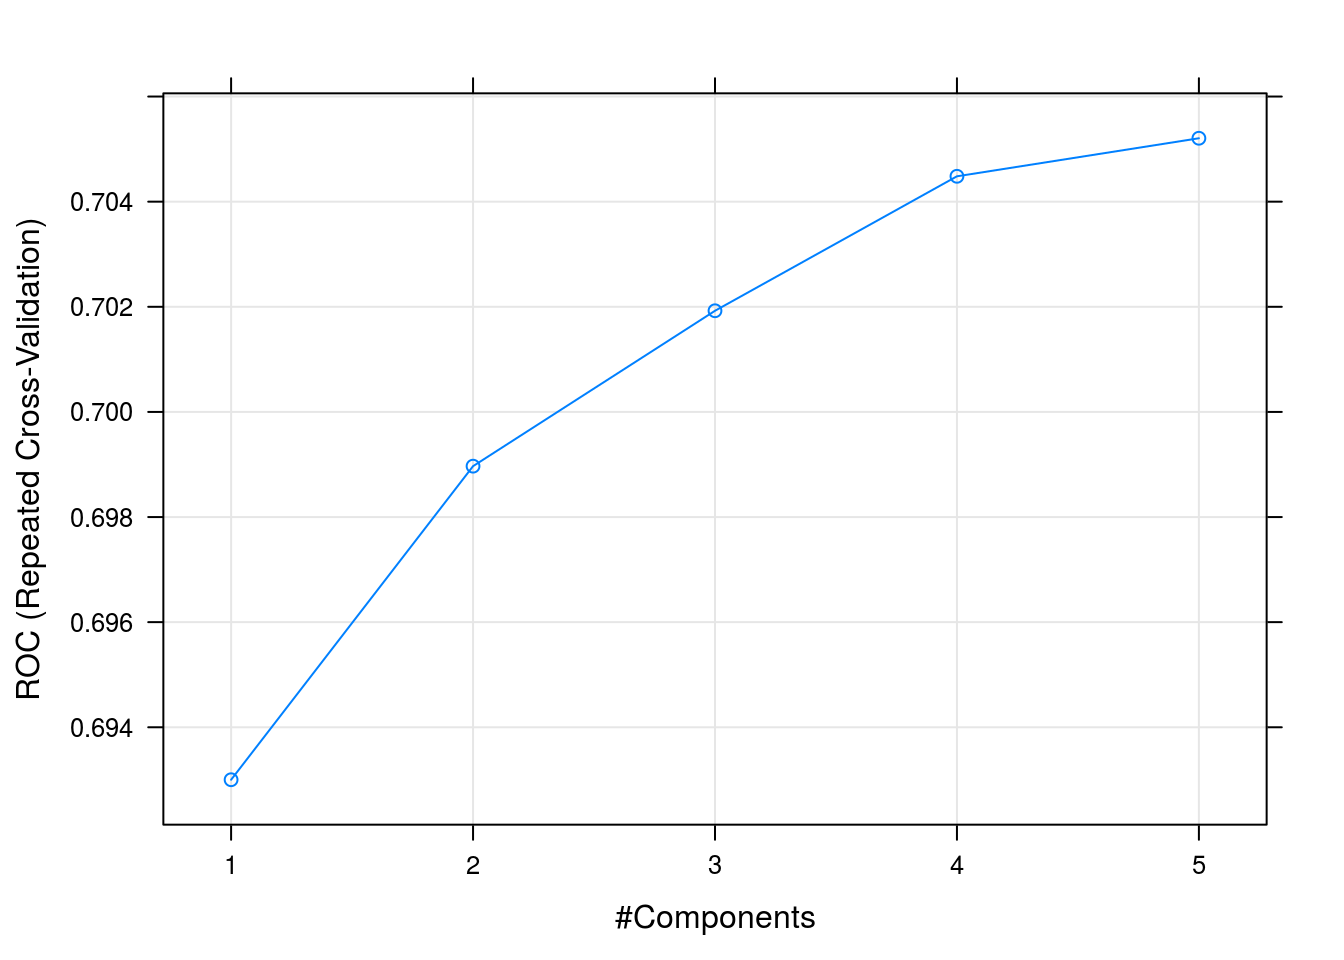
\includegraphics{DefectPredictionSoftEng_files/figure-latex/unnamed-chunk-12-1.pdf}

\begin{Shaded}
\begin{Highlighting}[]
\NormalTok{level_confidence <-}\StringTok{ }\FloatTok{0.95}
\NormalTok{repetitionsboot <-}\StringTok{ }\DecValTok{9999}
\NormalTok{samplemean <-}\StringTok{ }\NormalTok{function(x, d)\{}\KeywordTok{return}\NormalTok{(}\KeywordTok{mean}\NormalTok{(x[d]))\}}
\NormalTok{b_mean <-}\StringTok{ }\KeywordTok{boot}\NormalTok{(ae, samplemean, }\DataTypeTok{R=}\NormalTok{repetitionsboot)}
\NormalTok{confint_mean_China <-}\StringTok{ }\KeywordTok{boot.ci}\NormalTok{(b_mean)}
\end{Highlighting}
\end{Shaded}

\begin{verbatim}
## Warning in boot.ci(b_mean): bootstrap variances needed for studentized
## intervals
\end{verbatim}

\begin{Shaded}
\begin{Highlighting}[]
\NormalTok{confint_mean_China}
\end{Highlighting}
\end{Shaded}

\begin{verbatim}
## BOOTSTRAP CONFIDENCE INTERVAL CALCULATIONS
## Based on 9999 bootstrap replicates
## 
## CALL : 
## boot.ci(boot.out = b_mean)
## 
## Intervals : 
## Level      Normal              Basic         
## 95%   (1412, 2315 )   (1384, 2283 )  
## 
## Level     Percentile            BCa          
## 95%   (1451, 2350 )   (1486, 2419 )  
## Calculations and Intervals on Original Scale
\end{verbatim}

\begin{itemize}
\tightlist
\item
  Computing the bootstraped geometric mean
\end{itemize}

\begin{Shaded}
\begin{Highlighting}[]
\NormalTok{boot_geom_mean <-}\StringTok{ }\NormalTok{function(error_vec)\{}
  \NormalTok{log_error <-}\StringTok{ }\KeywordTok{log}\NormalTok{(error_vec[error_vec >}\StringTok{ }\DecValTok{0}\NormalTok{])}
  \NormalTok{log_error <-log_error[}\KeywordTok{is.finite}\NormalTok{(log_error)] }\CommentTok{#remove the -Inf value before calculating the mean, just in case}
  \NormalTok{samplemean <-}\StringTok{ }\NormalTok{function(x, d)\{}\KeywordTok{return}\NormalTok{(}\KeywordTok{mean}\NormalTok{(x[d]))\}}
  \NormalTok{b <-}\StringTok{ }\KeywordTok{boot}\NormalTok{(log_error, samplemean, }\DataTypeTok{R=}\NormalTok{repetitionsboot) }\CommentTok{# with package boot}
  \CommentTok{# this is a boot for the logs}
  \KeywordTok{return}\NormalTok{(b)}
\NormalTok{\}}
\CommentTok{# BCAconfidence interval for the geometric mean}
\NormalTok{BCAciboot4geommean <-}\StringTok{ }\NormalTok{function(b)\{  }
  \NormalTok{conf_int <-}\StringTok{ }\KeywordTok{boot.ci}\NormalTok{(b, }\DataTypeTok{conf=}\NormalTok{level_confidence, }\DataTypeTok{type=}\StringTok{"bca"}\NormalTok{)$bca }\CommentTok{#following 10.9 of Ugarte et al.'s book}
  \NormalTok{conf_int[}\DecValTok{5}\NormalTok{] <-}\StringTok{ }\KeywordTok{exp}\NormalTok{(conf_int[}\DecValTok{5}\NormalTok{]) }\CommentTok{# the boot was computed with log. Now take the measure back to its previous units}
  \NormalTok{conf_int[}\DecValTok{4}\NormalTok{] <-}\StringTok{ }\KeywordTok{exp}\NormalTok{(conf_int[}\DecValTok{4}\NormalTok{])}
  \KeywordTok{return} \NormalTok{(conf_int)}
\NormalTok{\}}
\CommentTok{# this is a boot object}
\NormalTok{b_gm <-}\StringTok{ }\KeywordTok{boot_geom_mean}\NormalTok{(ae) }\CommentTok{#"ae" is the absolute error in the China Test data}
\KeywordTok{print}\NormalTok{(}\KeywordTok{paste0}\NormalTok{(}\StringTok{"Geometric Mean of the China Test data: "}\NormalTok{, }\KeywordTok{round}\NormalTok{(}\KeywordTok{exp}\NormalTok{(b_gm$t0), }\DataTypeTok{digits=}\DecValTok{3}\NormalTok{)))}
\end{Highlighting}
\end{Shaded}

\begin{verbatim}
## [1] "Geometric Mean of the China Test data: 832.55"
\end{verbatim}

\begin{Shaded}
\begin{Highlighting}[]
\NormalTok{b_ci_gm <-}\StringTok{ }\KeywordTok{BCAciboot4geommean}\NormalTok{(b_gm)}
\KeywordTok{print}\NormalTok{(}\KeywordTok{paste0}\NormalTok{(}\StringTok{"Confidence Interval: "}\NormalTok{, }\KeywordTok{round}\NormalTok{(b_ci_gm[}\DecValTok{4}\NormalTok{], }\DataTypeTok{digits=}\DecValTok{3}\NormalTok{), }\StringTok{" - "}\NormalTok{, }\KeywordTok{round}\NormalTok{(b_ci_gm[}\DecValTok{5}\NormalTok{], }\DataTypeTok{digits=}\DecValTok{3}\NormalTok{)))}
\end{Highlighting}
\end{Shaded}

\begin{verbatim}
## [1] "Confidence Interval: 673.125 - 1009.427"
\end{verbatim}

\begin{Shaded}
\begin{Highlighting}[]
\CommentTok{# Make a % confidence interval bca}
\CommentTok{# BCAciboot <- function(b)\{  }
\CommentTok{#   conf_int <- boot.ci(b, conf=level_confidence, type="bca")$bca #following 10.9 of Ugarte et al.'s book}
\CommentTok{#   return (conf_int)}
\CommentTok{# \}}
\end{Highlighting}
\end{Shaded}

\chapter{Data Mining Issues in Defect
Prediction}\label{data-mining-issues-in-defect-prediction}

When dealing with imbalanced, there are some issues that need to be
taken into account.

\section{Unbalanced Datasets}\label{unbalanced-datasets}

Teachniques to deal with Imbalanced

\subsection{Subgroup discovery}\label{subgroup-discovery}

Subgroup Discovery (SD) aims to find subgroups of data that are
statistically different given a property of
interest\textasciitilde{}\citep{klosgen96,Wrobel97,Wrobel01,Herrera10}.
SD lies between predictive (finding rules given historical data and a
property of interest) and descriptive tasks (discovering interesting
patterns in data). An important difference with classification tasks is
that the SD algorithms only focus on finding subgroups (e.g., inducing
rules) for the property of interest and do not necessarily describe all
instances in the dataset.

In general, subgroups are represented through rules with the form
\{\(Cond \rightarrow Class\)\} having as consequent (\(Class\)) a
specific value of an attribute of interest. The antecedent (\(Cond\)) is
usually composed of a conjunction of attribute--value pairs through
relational operators. Discrete attributes can have the form of
\(att=val\) or \(att \neq val\) and for continuous attributes ranges
need to be defined, i.e., \(val_1 \leq att \leq val_2\).

\part{Bibliography}\label{part-bibliography}

\bibliography{references/dataSources.bib,references/SEmetrics.bib,references/RandStatistics.bib,references/referencesFS.bib,references/referencesIS.bib,references/RPackages.bib}


\end{document}
